\chapter{Modeling neurons}\label{sec:neurons}
The information processing in the brain is performed by neurons (see \cref{fig:neuron}).
Despite a wide variety of different neuron types and behaviours, the typical behavior of most neurons can be described as follows.
These cells build up an electrical potential of about \SI{-70}{\milli\volt}, the resting membrane potential, across their cell membrane with the ions in the intra- and extracellular fluid.
When the membrane potential is sufficiently depolarized (to about \SI{-50}{\milli\volt}), voltage gated ion channels will trigger a complete sudden and short-lived depolarization (typically about a \SI{1}{\milli\second}), a so called action potential or spike.
This action potential will travel along the neuron's axon and trigger the release of neurotransmitters at its synapses where it connects to other neuron's dendrites.
The released neurotransmitters will influence the ion channels of the post-synaptic neuron and either lower (inhibitory synapse) or raise (excitatory synapse) the membrane potential.
The deflection of the membrane potential depends on the strength of the synapse and the speed of the release and uptake of the neurotransmitter.
If the post-synaptic neuron receives sufficient input from other neurons, its membrane potential will be sufficiently deflected to initiate a new action potential.
By the pattern of connectivity that controls what activity in some neurons triggers activity in other neurons, the brain is able to perform the computations that lead to an animal's or human's behavior.

\begin{figure}
    \centering
    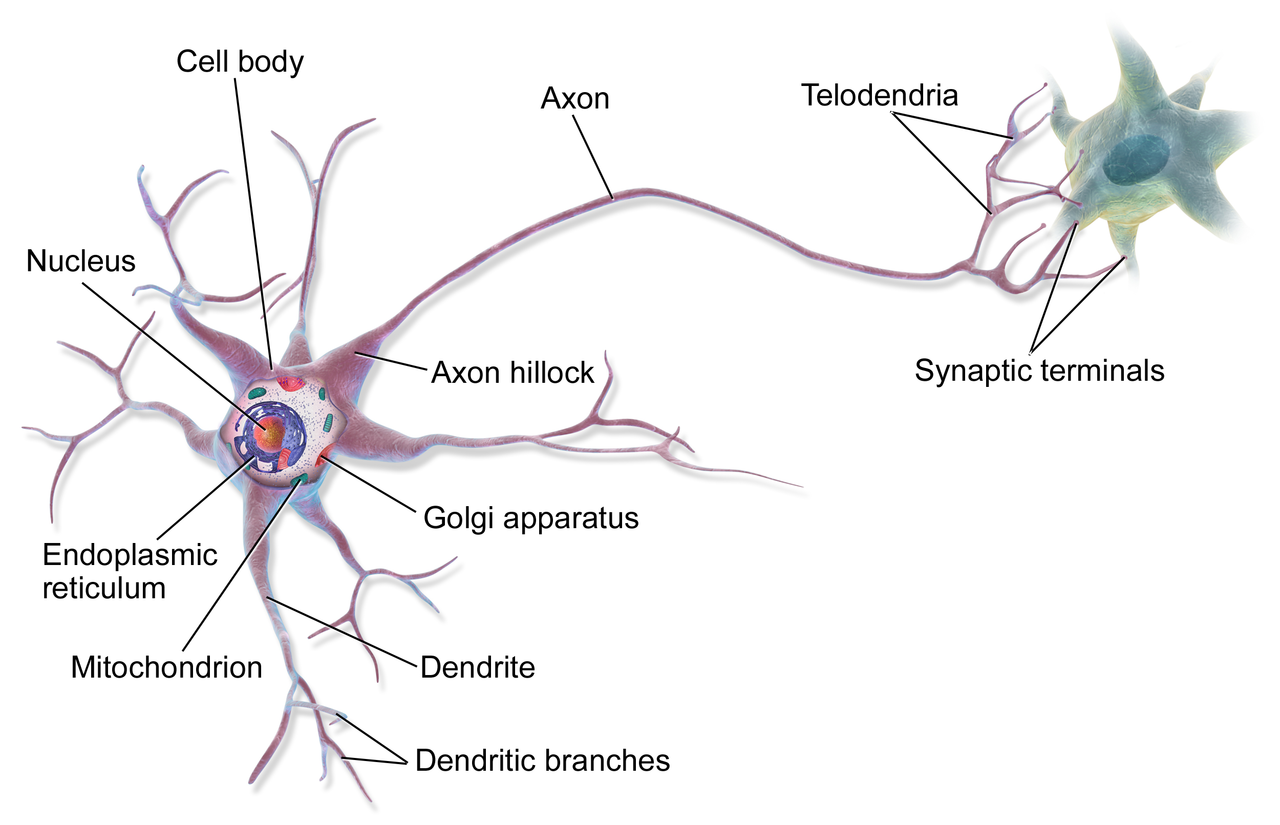
\includegraphics[width=0.8\textwidth]{figures/Blausen_0657_MultipolarNeuron}
    \caption[A typical neuron]{A typical neuron. Image by Blausen Medical Communications, Inc.\ and reused under the Creative Commons Attribution 3.0 Unported license.}\label{fig:neuron}
\end{figure}

To computationally model neurons, it is necessary to chose a level of abstraction.
On the one hand, it is possible to create very detailed models with spatial extent \parencite[e.g.,][]{markram2015,bahl2012} where individual ion channels and the propagation of electrical potentials is modeled.
On the other hand, one can use very abstract neuron models that basically consist of nodes summing their inputs and applying non-linearity using real valued stand-ins for firing rates (instead of discrete spikes).
This latter type of model is common in artificial neural networks and deep learning.

A widely used neuron model in computational neuroscience is the leaky integrate-and-fire (LIF) neuron model.
It is a point neuron model, thus not modeling any spatial extend.
It models a single membrane voltage $V(t)$ described by the differential equation
\begin{equation}
    \taurc \od{V}{t} = -V(t) + R J(t)
\end{equation}
where $R$ is the membrane resistance, $J(t)$ the input current, and $\taurc$ the membrane time constant.
Whenever the membrane voltage reaches a certain threshold $V_{\ped{th}}$, the LIF neuron transmits a spike and its membrane voltage is reset for a refractory period of $\tauref$.
This type of neuron model allows to derive the firing rate for a given constant input current $J$ analytically as
\begin{equation}
    \act(J) = \frac{1}{\tauref - \taurc \ln\!\del{1 - \frac{V_{\ped{th}}}{R J}}} \text{.}
\end{equation}

The LIF neuron model is a good choice for the undertaking of this thesis as it captures many aspects of neuron behavior.
It is detailed enough to relate parameters like the membrane time constant to the actual biological correspondents.
This allows to fix these parameters to values within the biological plausible range instead of having them as free parameters in the model that would require parameter matching and give the model additional degrees of freedom to match the data.
At the same time the model is simple enough to allow for reasonable performance when simulating large-scale models with these neurons.
